%%
%% This is file `sample-manuscript.tex',
%% generated with the docstrip utility.
%%
%% The original source files were:
%%
%% samples.dtx  (with options: `manuscript')
%% 
%% IMPORTANT NOTICE:
%% 
%% For the copyright see the source file.
%% 
%% Any modified versions of this file must be renamed
%% with new filenames distinct from sample-manuscript.tex.
%% 
%% For distribution of the original source see the terms
%% for copying and modification in the file samples.dtx.
%% 
%% This generated file may be distributed as long as the
%% original source files, as listed above, are part of the
%% same distribution. (The sources need not necessarily be
%% in the same archive or directory.)
%%
%% The first command in your LaTeX source must be the \documentclass command.
%%%% Small single column format, used for CIE, CSUR, DTRAP, JACM, JDIQ, JEA, JERIC, JETC, PACMCGIT, TAAS, TACCESS, TACO, TALG, TALLIP (formerly TALIP), TCPS, TDSCI, TEAC, TECS, TELO, THRI, TIIS, TIOT, TISSEC, TIST, TKDD, TMIS, TOCE, TOCHI, TOCL, TOCS, TOCT, TODAES, TODS, TOIS, TOIT, TOMACS, TOMM (formerly TOMCCAP), TOMPECS, TOMS, TOPC, TOPLAS, TOPS, TOS, TOSEM, TOSN, TQC, TRETS, TSAS, TSC, TSLP, TWEB.
% \documentclass[acmsmall]{acmart}

%%%% Large single column format, used for IMWUT, JOCCH, PACMPL, POMACS, TAP, PACMHCI
% \documentclass[acmlarge,screen]{acmart}

%%%% Large double column format, used for TOG
% \documentclass[acmtog, authorversion]{acmart}

%%%% Generic manuscript mode, required for submission
%%%% and peer review
\documentclass[manuscript,screen]{acmart}

%%
%% \BibTeX command to typeset BibTeX logo in the docs
\AtBeginDocument{%
  \providecommand\BibTeX{{%
    \normalfont B\kern-0.5em{\scshape i\kern-0.25em b}\kern-0.8em\TeX}}}

%% Rights management information.  This information is sent to you
%% when you complete the rights form.  These commands have SAMPLE
%% values in them; it is your responsibility as an author to replace
%% the commands and values with those provided to you when you
%% complete the rights form.
\setcopyright{acmcopyright}
\copyrightyear{2018}
\acmYear{2018}
\acmDOI{10.1145/1122445.1122456}

%% These commands are for a PROCEEDINGS abstract or paper.
\acmConference[Woodstock '18]{Woodstock '18: ACM Symposium on Neural
  Gaze Detection}{June 03--05, 2018}{Woodstock, NY}
\acmBooktitle{Woodstock '18: ACM Symposium on Neural Gaze Detection,
  June 03--05, 2018, Woodstock, NY}
\acmPrice{15.00}
\acmISBN{978-1-4503-XXXX-X/18/06}


%%
%% Submission ID.
%% Use this when submitting an article to a sponsored event. You'll
%% receive a unique submission ID from the organizers
%% of the event, and this ID should be used as the parameter to this command.
%%\acmSubmissionID{123-A56-BU3}

%%
%% The majority of ACM publications use numbered citations and
%% references.  The command \citestyle{authoryear} switches to the
%% "author year" style.
%%
%% If you are preparing content for an event
%% sponsored by ACM SIGGRAPH, you must use the "author year" style of
%% citations and references.
%% Uncommenting
%% the next command will enable that style.
%%\citestyle{acmauthoryear}

%%
%% end of the preamble, start of the body of the document source.
\begin{document}

%%
%% The "title" command has an optional parameter,
%% allowing the author to define a "short title" to be used in page headers.
\title{Spatiotemporal-Aware Visualizations in Augmented Reality Music Teaching Systems}

%%
%% The "author" command and its associated commands are used to define
%% the authors and their affiliations.
%% Of note is the shared affiliation of the first two authors, and the
%% "authornote" and "authornotemark" commands
%% used to denote shared contribution to the research.
\author{Jordan Aiko Deja}
%\authornote{Both authors contributed equally to this research.}
\email{jordan.deja@famnit.upr.si}
\orcid{1234-5678-9012}
\affiliation{%
  \institution{University of Primorska}
  \city{Koper}
  \country{Slovenia}
  \postcode{6000}
}

\author{Matjaž Kljun}
\affiliation{%
  \institution{University of Primorska}
  \city{Koper}
  \country{Slovenia}
  \postcode{6000}}
\email{matjaz.kljun@famnit.upr.si}

\author{Klen Čopič Pucihar}
\affiliation{%
  \institution{University of Primorska}
  \city{Koper}
  \country{Slovenia}
  \postcode{6000}}
\email{klen.copic@famnit.upr.si}

%%
%% By default, the full list of authors will be used in the page
%% headers. Often, this list is too long, and will overlap
%% other information printed in the page headers. This command allows
%% the author to define a more concise list
%% of authors' names for this purpose.
\renewcommand{\shortauthors}{Deja, et al.}

%%
%% The abstract is a short summary of the work to be presented in the
%% article.
\begin{abstract}
  Spatiotemporal interactions refer to a range of interactive activities that take place in a particular space at a particular time. The spatiotemporal component in extended reality (XR) allows users to interact with or act based on moving digital elements and visualisations within a particular time frame such as pointing to a moving target, button-clicking, or batting a flying baseball. In such scenarios, users only have a dedicated time window to sense (perceive) the movement of digital elements/visualisations, recognise them, decide on the appropriate response and act accordingly in relation to the moving target. The research on XR spatiotemporal interactions has focused on modelling error rates in spatiotemporal pointing, which allowed designers to mitigate and prevent user errors. However, more work is needed to understand XR spatiotemporal interactions in specific contextualised environments such as XR music teaching systems. AR music teaching systems usually rely on visualisations and other similar cues to help novices learn a specific instrument or a musical piece. These studies have not modeled spatiotemporal interaction as well and have not taken into account psycho cognitive responses. This research proposal attempts to understand the role of spatiotemporal interactions in XR music teaching systems for experts and novices. User learning habits, instrument playing patterns and cognitive load will be investigated, observed and will be used to build models in order to design spatiotemporal-aware visualisations, which can enhance music learning experience. 
\end{abstract}

%%
%% The code below is generated by the tool at http://dl.acm.org/ccs.cfm.
%% Please copy and paste the code instead of the example below.
%%
\begin{CCSXML}
<ccs2012>
 <concept>
  <concept_id>10010520.10010553.10010562</concept_id>
  <concept_desc>Computer systems organization~Embedded systems</concept_desc>
  <concept_significance>500</concept_significance>
 </concept>
 <concept>
  <concept_id>10010520.10010575.10010755</concept_id>
  <concept_desc>Computer systems organization~Redundancy</concept_desc>
  <concept_significance>300</concept_significance>
 </concept>
 <concept>
  <concept_id>10010520.10010553.10010554</concept_id>
  <concept_desc>Computer systems organization~Robotics</concept_desc>
  <concept_significance>100</concept_significance>
 </concept>
 <concept>
  <concept_id>10003033.10003083.10003095</concept_id>
  <concept_desc>Networks~Network reliability</concept_desc>
  <concept_significance>100</concept_significance>
 </concept>
</ccs2012>
\end{CCSXML}

\ccsdesc[500]{Computer systems organization~Embedded systems}
\ccsdesc[300]{Computer systems organization~Redundancy}
\ccsdesc{Computer systems organization~Robotics}
\ccsdesc[100]{Networks~Network reliability}

%%
%% Keywords. The author(s) should pick words that accurately describe
%% the work being presented. Separate the keywords with commas.
\keywords{datasets, neural networks, gaze detection, text tagging}


%%
%% This command processes the author and affiliation and title
%% information and builds the first part of the formatted document.
\maketitle

\section{Introduction}
Spatiotemporal interactions in immersive environments such as virtual, augmented and mixed reality systems (umbrella term for these is extended reality (XR)) refer to a range of user activities that users need to perform in relation to both time and space. Temporal interaction requires users’ actions within a particular time window in response to an event taking place. For example, several recent studies have explored temporal pointing \cite{lee2016modelling} defined as interaction in which users need to provide discrete input (e.g., button press), with no or negligible spatial aiming demand (the finger is on the button) in a particular time window (usually very short). Spatial interaction requires users to complete an action at a particular place in space. In contrast to temporal pointing, spatial pointing requires users to aim at a fixed or moving target in space while time is not predefined (e.g. just as quickly as possible). As such, spatiotemporal pointing combines these two principles and is referred to as the user action in an immersive environment as a response to a temporarily available digital stimulus. Examples of spatiotemporal interactions include batting a virtual baseball in a XR environment or hitting the right keys at the right time in an XR piano teaching system. In both examples users need to point to a precise location (hitting the ball with a controller representing the virtual bat or pressing the piano key) at the right time. \\

To be able to complete such spatiotemporal pointing \cite{lee2016modelling}, users have an internal time-keeping mechanism to synchronise their movements to an external stimulus according to the WK model \cite{wing1973response}. Additionally, a response-execution stage that allows the user to process input-stimulus and output-actions, is also needed \cite{wing1973timing}. Other studies have focused on (i) investigating and understanding human cognitive load \cite{radu2009augmented}, (ii) improving the accuracy in the rendering of visual elements (which is also referred to as spatial registration \cite{zheng2013general}), and (iii) discovering novel approaches to minimise latency of visualising overlaying digital visualisations \cite{serafin2017considerations}. \\

Innovations in spatiotemporal interactions also directly contribute to computational human-computer interaction (HCI). The concept of computational HCI considers usage of explicit mathematical models of user-system behavior in order to influence, automate and improve the design process of a system. For example, the collected user data can directly feed back into a model, improving the behaviour of the targets of spatiotemporal interaction. Since extended reality environments present an ideal space to investigate spatiotemporal pointing, we push our contributions further by incorporating techniques in computational HCI. Several formative studies have focused on modelling, predicting, and simulating action and reaction in such environments. These studies have contributed to understanding of (1) how objects move and collide in virtual spaces \cite{lee2017boxer}, (2) how users respond to these objects \cite{lee2016modelling} and (3) how we can foster design affordances that improve their performance \cite{rogers2014piano}.\\

Our work will focus on investigating spatiotemporal pointing in XR environments and the design of such systems based on computational HCI by exploring augmented reality (AR) music teaching systems - specifically a piano teaching system. Several such systems have been built with augmented and virtual reality as a medium for innovation by overlaying augmented time-specific visualisations over piano keys to improve music learning experiences \cite{rogers2014piano, sun2018mr, birhanu2017keynvision}. However, cognitive load and user response times have not been observed and taken into account. Moreover, these prototypes were not based on the pre-built spatiotemporal pointing model. Our research will fill this gap by designing spatiotemporal-aware visualisations based on the pre-built models that take user-data into account, which will in our opinion improve  AR piano learning experiences. \\

\section{Related Work}
This section will discuss studies on spatial and temporal interactions on screen and in extended reality (XR) environments followed by the section describing piano teaching systems that use AR visualisations. 

\subsection{Studies on modeling spatiotemporal interactions}
Here we present a few studies in temporal and spatiotemporal pointing and error predicting models. Spatiotemporal pointing has been so far mostly investigated outside augmented reality (AR) by modeling, analysing and predicting user error rates. Exploring spatiotemporal pointing in AR is relatively new, while exploration of modeling spatiotemporal pointing in AR music learning is, to the best of our knowledge, nonexistent. We will take the knowledge presented into account, build models for AR music learning and explore spatiotemporal pointing in these settings.

\begin{figure}[t]
\centering
 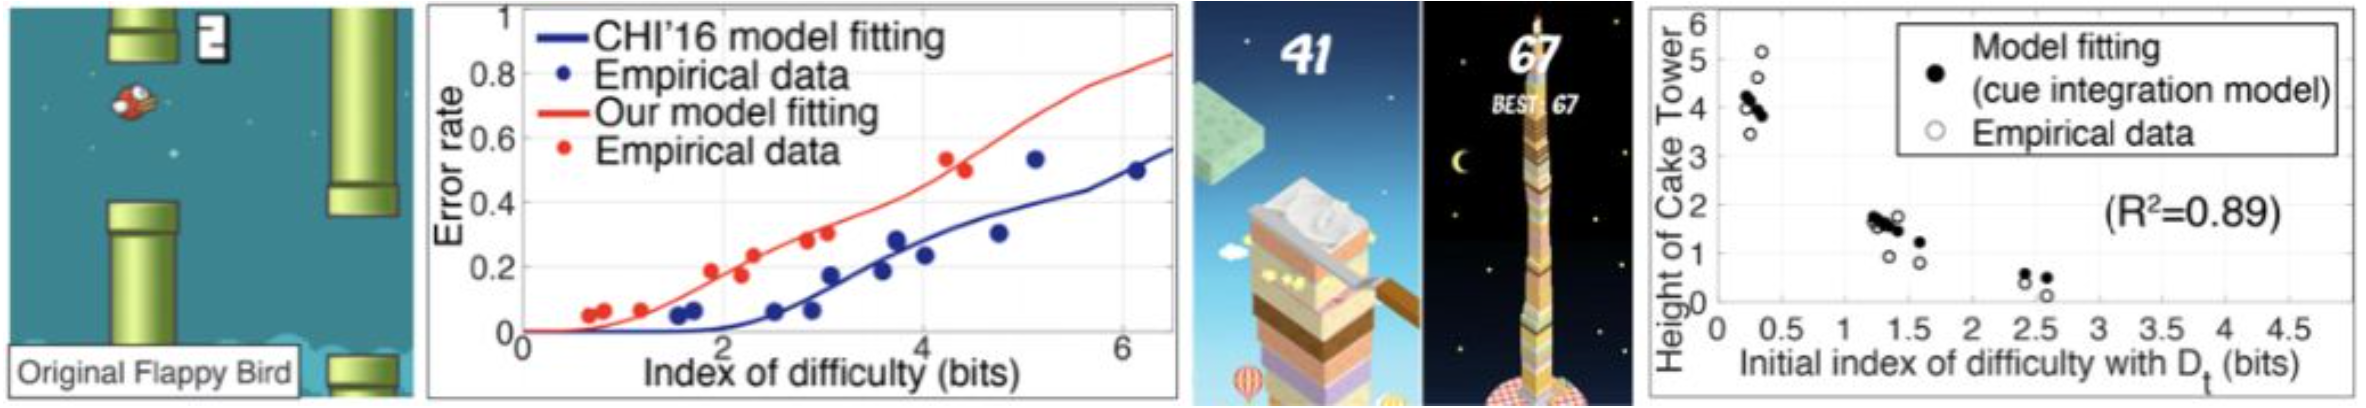
\includegraphics[width=12cm]{figures/flappybird.png}
    \caption{Temporal pointing models could predict player scores and error rates for one-button games such as Flappy Bird (left) and Cake Tower (right).
    }\label{fig:flappybird}
\end{figure}

\begin{itemize}
\item The study of \citeA{lee2016modelling} and \citeA{lee2018moving} built models to predict players’ performance and error rates in some real-time games that are played with a single button — temporal pointing. Their model could successfully predict the players’ performance while playing popular games such as Flappy Bird and Cake Tower (see Figure \ref{fig:flappybird}). The presented model can be applied to adaptively change a game’s difficulty level according to changes in the system (change in latency or speed of moving objects). \\
\item The study of \citeA{lee2017boxer} investigated collision events in a virtual scene from throwing, pushing or pulling an object.  In their prototype called Boxer users received a salient sensory feedback when a pointer (a hand in this study) made contact with a moving object (a virtual ball) — more precisely the prototype triggered. The prototype allows a collision when the pointer reaches a minimum speed after first contact between the object and the pointer. They compared this spatiotemporal pointing with a temporal pointing (just pressing a button) presented in the study described above. Based on their findings, spatial precision in collisions improved by 26.7\%. It was also reported that accuracy can be compromised under specific user task conditions. Their study also reported that there were no observed differences in temporal precision. \\
\item The work of \citeA{kim2018impact} presented an activation technique called Impact Activation (IA). This describes the point where a button is activated at its maximal impact point. Based on their findings, IA as a technique is most useful during particularly-rapid repetitive button pressing activities which are usually observed in games and music applications. While their study focused more on rapid button pressing, their findings were able to report on user’s timing accuracy and how they improved significantly by using impact activation. The proposed technique can be implemented in modern push-button setups that generate a continuous signal. In music teaching systems, pressing the piano key resembles an action of pressing a button. Users pressing on a setup like a piano teaching system may potentially take advantage from accuracy improvements that use impact activation. 
\end{itemize}

\begin{figure}[t]
\centering
 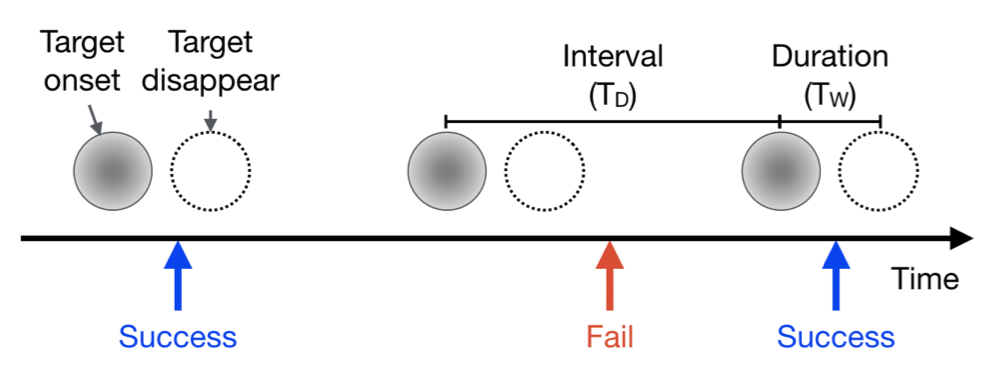
\includegraphics[width=8cm]{figures/boxmodel.png}
    \caption{One of the timing experiments with a box model done by Lee. It considers capturing timing error while the user attempts to catch a target that is regularly blinking.
    }\label{fig:boxmodel}
\end{figure}

\subsection{Studies on music teaching systems, augmented reality and visualizations}

\begin{figure}[h]
\centering
 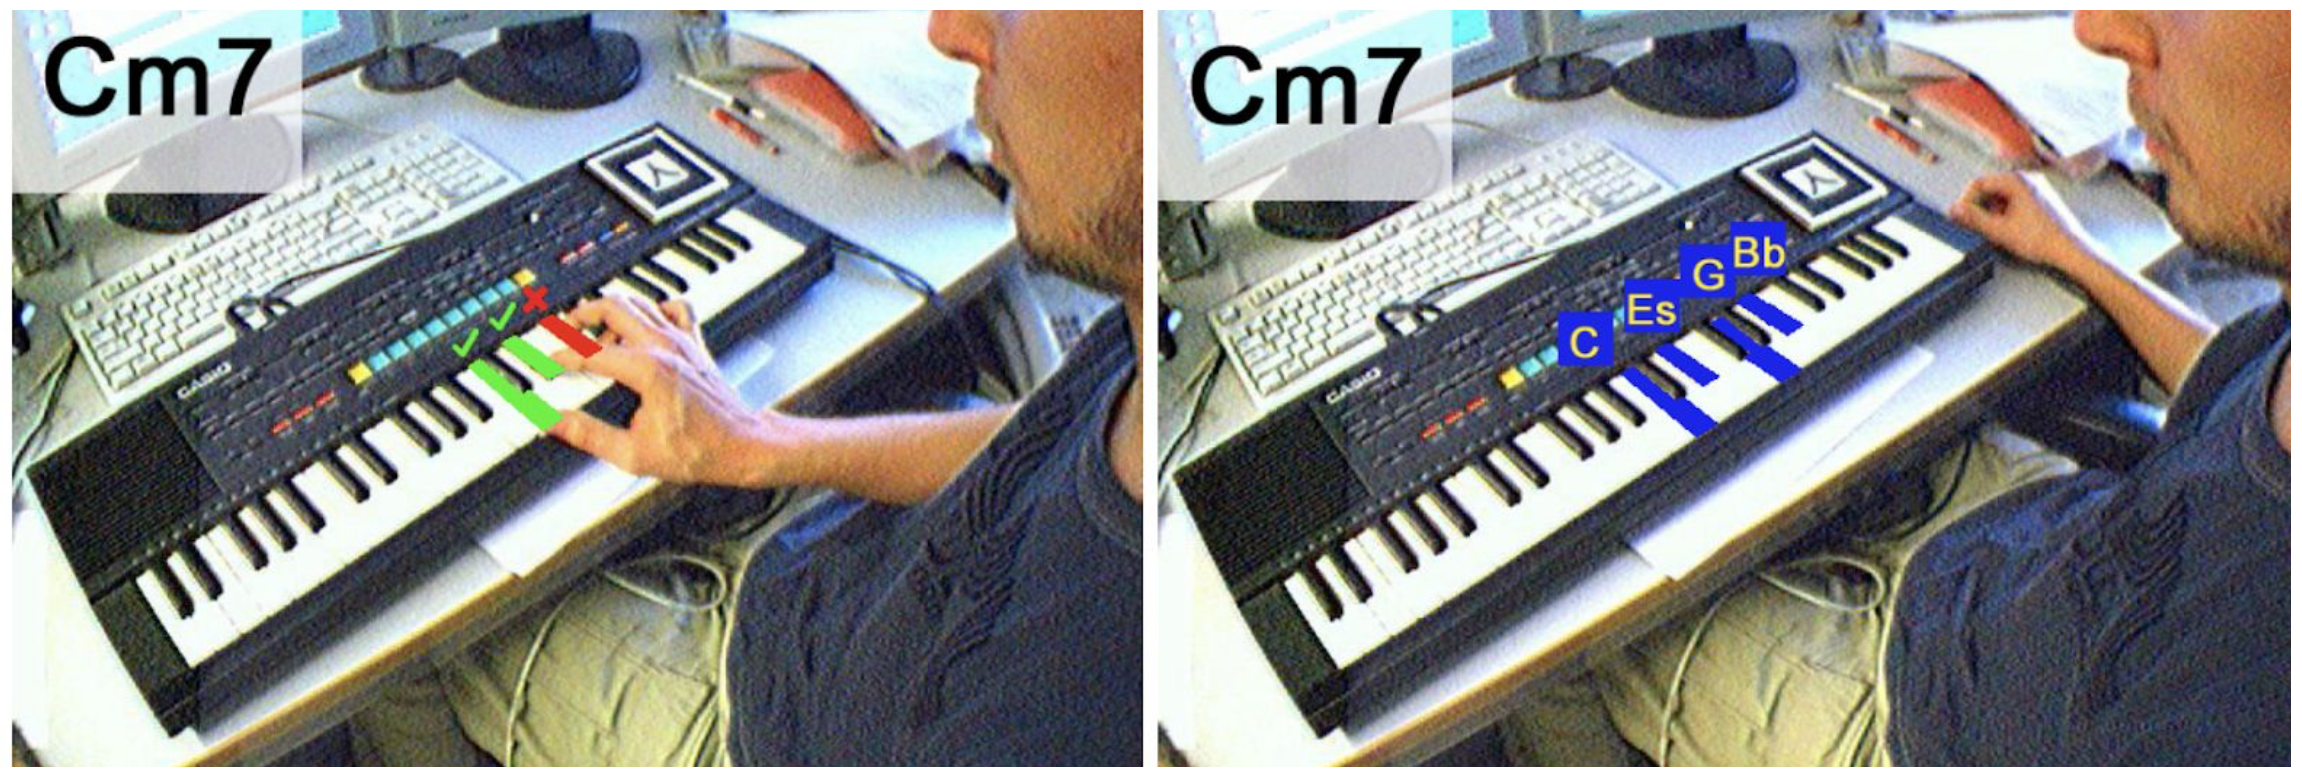
\includegraphics[width=12cm]{figures/barakonyi.png}
    \caption{Prototype by Brakonyi. Visualisations are seen overlying the keys of the MIDI keyboard.
    }\label{fig:barakonyi}
\end{figure}

Computer assisted music teaching systems date back to the early 2000’s. Here we present a few examples. Most of the recent contributions in AR music teaching systems focus on either (1) introducing novel interfaces \cite{barakonyi2005augmented, huang2011piano}, (2) different learner modes for the users \cite{weing2013piano, rogers2014piano}, and (3) improving graphical rendering of the visualisations \cite{chow2013music, zheng2013general}. None of them took users’ cognitive load and response times into account, and were not based on the pre-built spatiotemporal pointing model in order to better support piano learning processes based on users’ performance. Our research will fill this gap by designing spatiotemporal-aware visualisations based on the pre-built models that take user-data into account, which will in our opinion improve AR piano learning experiences.\\

\begin{figure}[h]
\centering
 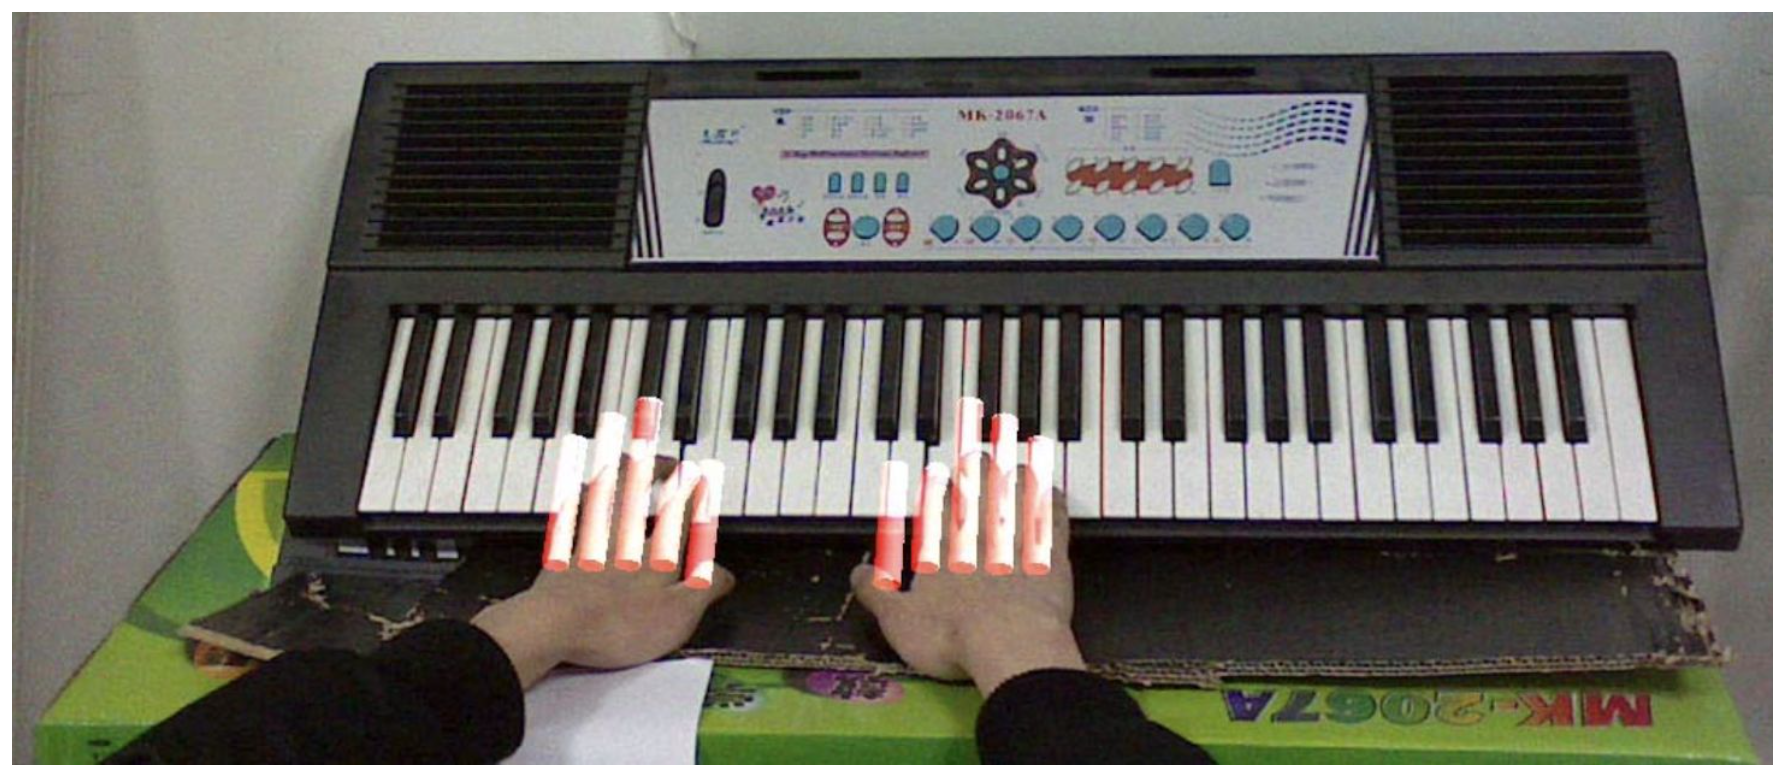
\includegraphics[width=12cm]{figures/huang.png}
    \caption{Prototype by Huang. The virtual hands are seen as overlaid the fingers and keys on the keyboard.
    }\label{fig:huang}
\end{figure}
\begin{figure}[h]
\centering
 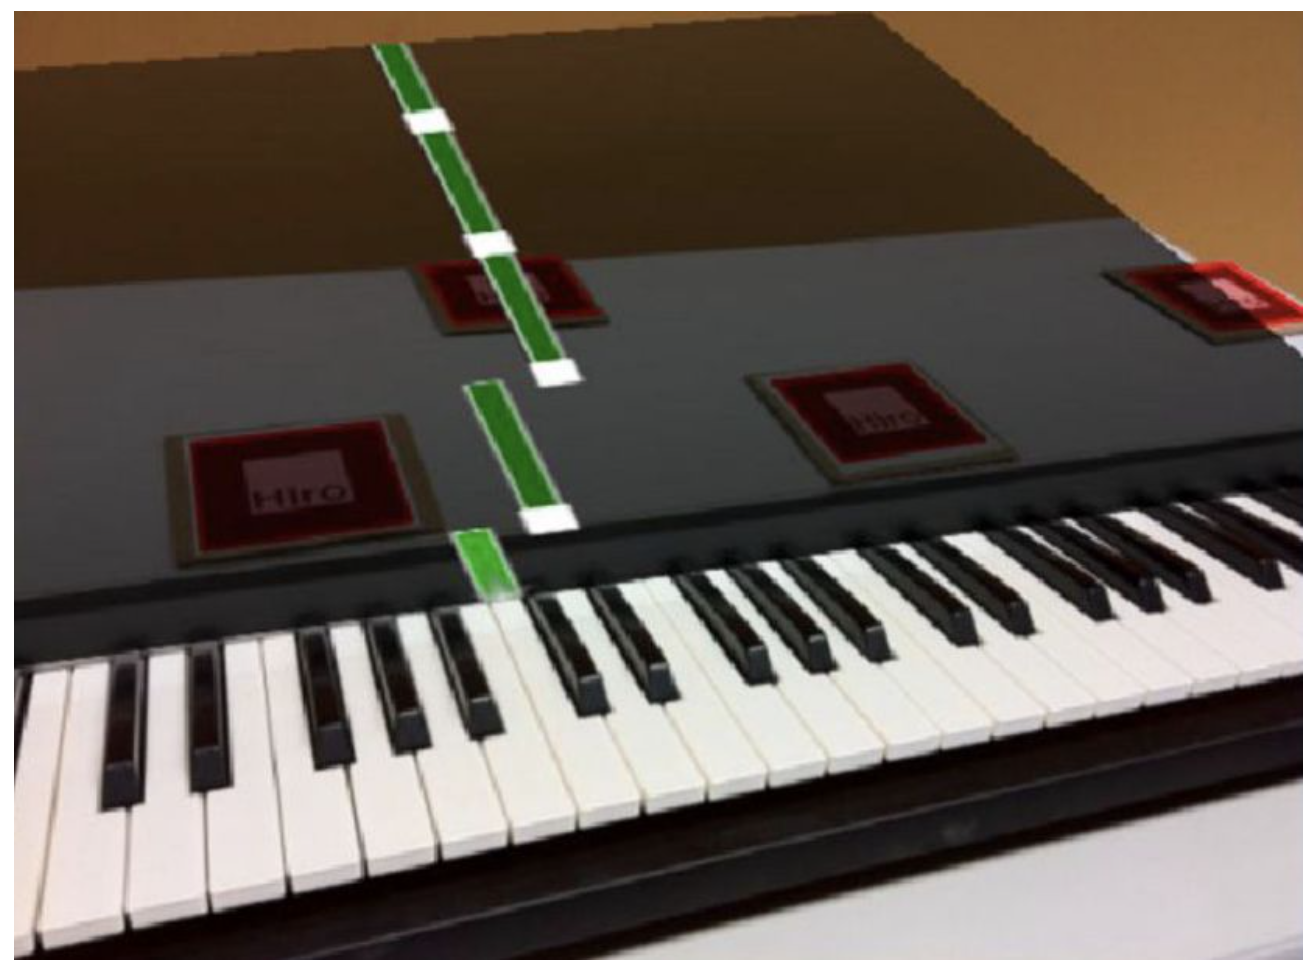
\includegraphics[width=12cm]{figures/chow.png}
    \caption{Prototype by Chow. A piano roll visualisation is seen as “falling notes” in the visualisations.
    }\label{fig:chow}
\end{figure}

\begin{itemize}
\item The work of \citeA{barakonyi2005augmented} presented an AR piano tutor seen in Figure 3. The prototype used a webcam, a monitor and a MIDI keyboard. The webcam captured the keyboard that was shown on the monitor together with digital information instructing users to hit certain keys in a defined order as well as giving audio feedback as to which keys have been pressed correctly and which were pressed by mistake. The system also included an advanced music composition tool by analysing the tunes currently being played and suggesting background chords and appropriate solo melodies.\\
\item The prototype of \citeA{huang2011piano} presented a markerless AR based piano teaching system. It used virtual hands overlaid on a real keyboard \ref{fig:huang} which allowed piano beginners to practice playing the piano. The technology presented in this paper focuses on the tracking of the real keyboard and overlying of virtual hands and not on the learning music.\\
\item The prototype by \citeA{chow2013music} presents an AR prototype using a head mounted display. The prototype is targeting people who practice the instrument on their own (how it is done traditionally) and lack feedback on how to improve their playing as well as motivation for learning. Their prototype addressed these two shortcomings by visualising “falling” notes as seen in Figure \ref{fig:chow} providing direct feedback, and including game elements to learning. The findings show that beginners improved their notation literacy.\\
\item The work of \citeA{weing2013piano} presents a prototype that enhances musical instrument learning with projected visualisations. Their P.I.A.N.O. prototype \ref{fig:ubicomp} aims to support learning to play a piano by considering the learning curve of beginners and addressing hard-to-learn music notations. These notations are replaced by an alternative representation, which are projected onto the piano. Aside from the design of a piano prototype with interactive visualisations and projections, their study also proposed three different learning modes that support novice learners (listen, practice, play modes). They were able to improve on top of the work of \citeA{chow2013music} by using gamification and interactivity to prolong student motivation. The P.I.A.N.O. was improved further in \citeA{rogers2014piano} by mapping the correct visualisations with extra articulation or enhanced piano roll notation as referred to by authors. Their findings measured (i) significantly lower cognitive load, (ii)  improved user experience, and (iii) an increase in perceived music quality rated by the experts as compared against non-projected piano roll notation. \\
\end{itemize}
\begin{figure}[h]
\centering
 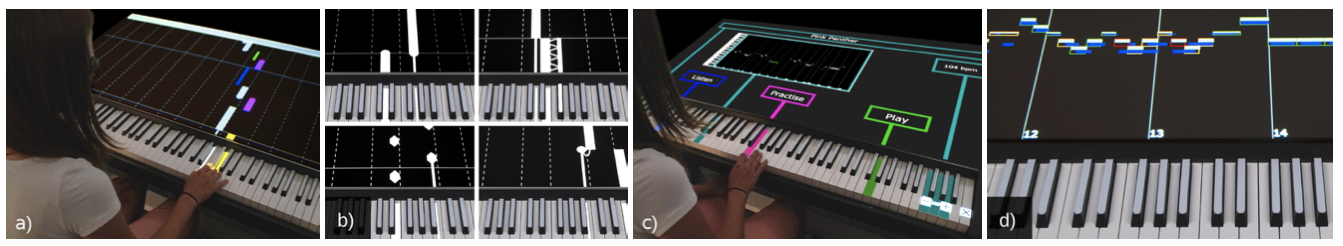
\includegraphics[width=12cm]{figures/pianoUBC.png}
    \caption{Photos of the P.I.A.N.O. interface by Rogers. It included overlaid visualizations, practice modes and detailed feedback. 
    }\label{fig:ubicomp}
\end{figure}
The works of \citeA{liao2020button, lee2019geometrically, arora2019magicalhands} have laid the groundwork on modeling and measuring spatiotemporal pointing in augmented reality systems. They did modelling experiments on pressing a button, batting a virtual baseball and authoring animations using gestures in an augmented reality space. This research will focus on understanding spatiotemporal pointing and their user models in augmented reality music teaching systems. This research will consider the steps on how to build and analyze these models towards better understanding expert and novice musicians. The cognitive load that measures their learning in augmented reality will also be measured along with spatiotemporal pointing data. This research introduces spatiotemporal-aware visualizations that consider both psycho cognitive factors and spatiotemporal data. The findings of the proposed research will be very useful to the research community interested in augmented reality, music teaching systems, interface  and visualization design.\\

\section{Research Plan and Research Method}
The focus of this research will be on exploring the AR piano teaching system based on the general research question: “How to  build models of interactions of experts and novices in AR piano teaching systems and use them to design spatiotemporal-aware visualisations that can help novices in their music learning experiences?”. The models will allow us to understand the differences between the way experts and novices use the developed system while the collected interaction patterns and insights around them will be used to design better visualisations.\\

The detailed research questions and the research plan are presented in the following subsections. 

\subsection{Research Questions}
Our research is guided by the following research questions: 
\begin{enumerate}
    \item How do we model expert and novice spatiotemporal interactions with various musical instruments (guitar, piano, xylophone) with augmented reality? \\
    Hypothesis: We can use earlier studies on spatiotemporal pointing in augmented reality  to build expert and novice models on augmented reality music teaching systems. From these models, we can see differences in their spatiotemporal interactions.  
    \item Is there a relationship between spatiotemporal pointing and psycho cognitive responses when using augmented reality music teaching systems? \\
    Hypothesis: There is a link between spatiotemporal pointing and psycho cognitive responses when interacting with visualizations in augmented reality music teaching systems. Models from expert users can then be used as a baseline in helping novice users. 
    \item What features of spatiotemporal-aware visualizations in augmented reality music teaching systems can we introduce to help novice users?\\
    Hypothesis: Designing visualizations that consider both, spatiotemporal interaction models, and psycho cognitive load of its users,  can in turn,  improve the learning curve of novices and their user experiences in augmented reality piano teaching systems. 
    \item Can novices adapt and learn better with spatiotemporal-aware visualizations in augmented reality piano teaching systems? \\
    Hypothesis: Novices adapt and interact easily if the visualizations that guide them in AR piano teaching systems are spatiotemporal-aware.
    \item How can we design and deploy an ubiquitous augmented reality piano teaching system that uses spatiotemporal-aware visualizations?\\
    Hypothesis: The effects of spatiotemporal-aware visualizations can be used in an ubiquitous interface that can provide better user experience and learner flexibility. 

\end{enumerate}
Spatiotemporal pointing has been widely-used outside augmented reality. Several studies have done modeling, analyzing and predicting error rates. The same set of studies in augmented reality are relatively new and there is much room to explore. Existing HCI work attempts to understand and model human interactions while doing activities with augmented reality music teaching systems.\\

Most of the recent contributions in augmented reality music teaching systems focus on either (1) introducing a new ubiquitous interface, (2) having different learner modes for the users, and (3) improving graphical rendering of the visualizations. Studies that investigate and model spatiotemporal pointing on augmented reality music teaching systems are very limited. This will be the intended focus of this research. \\
We ask the general research question: “How might we model the interactions of experts and novices when using augmented reality music teaching systems and use them to design spatiotemporal-aware visualizations that can help novices in their music learning experiences?”. We use this general research question as the basis for our hypothesis statements. \\

We can model the spatiotemporal pointing activities of both novices and expert users while using augmented reality music teaching systems. We believe that these models will allow us to understand the differences between the way experts and novices use these systems. With this, we will look into their patterns and the insights around them, which in turn we can use to design better visualizations. An overview of the research plan is described in Fig 4. The green branches show a set of experiments that aim to investigate the specific HCI application areas in relation to spatiotemporal pointing and augmented reality music teaching systems (piano, guitar, xylophone, etc). The orange branches show a range of setups that combine results from the experiments done in the green branches, and in relation to sensorimotor and psychophysics, bridging cognitive load and user models. Results of the experiments from the orange and green branches will provide groundwork for this research. The middle branch is the main focus of this thesis. It will focus mainly on augmented reality piano teaching systems. It will investigate the differences between the spatiotemporal models of novices and experts while using these systems. \\
\begin{landscape}
\begin{figure}[h]
\centering
 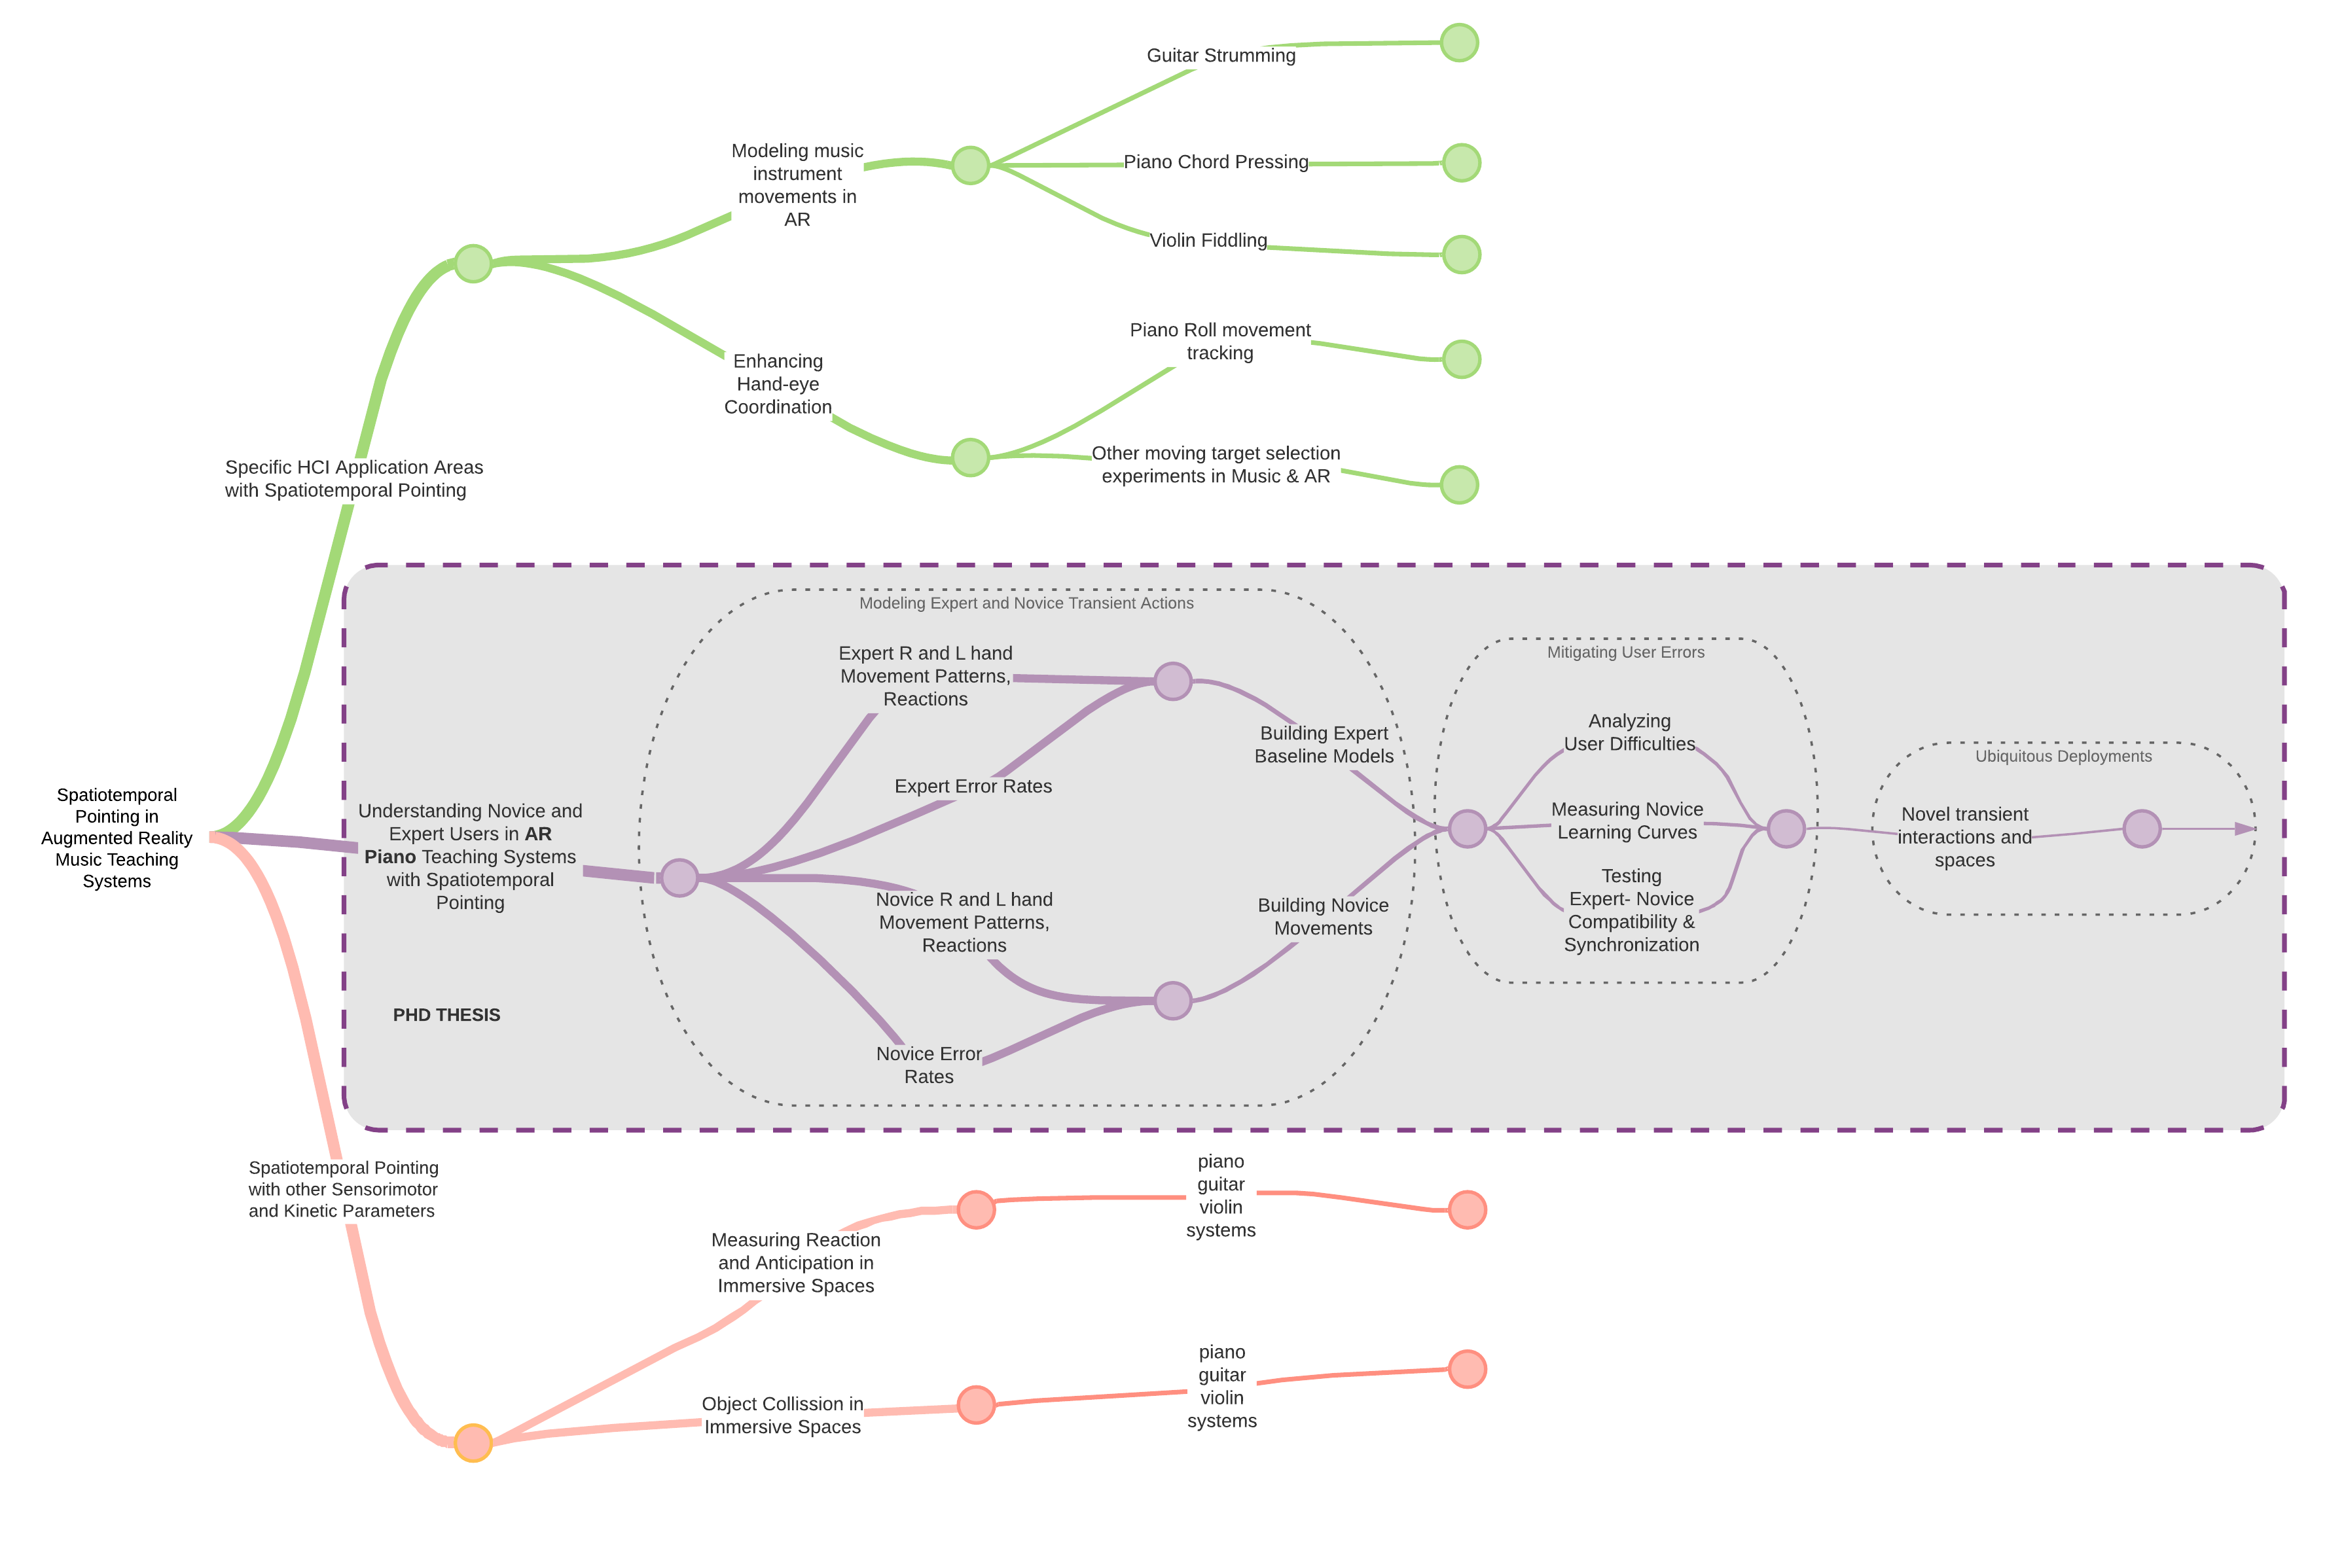
\includegraphics[width=\columnwidth\textheight]{figures/branches.png}
    \caption{An overview of the research branches showing breadth and depth. Each branch represents an experiment which will be part of the methodology in this proposal. Each node in the diagram is targetted  as a concrete contribution leading to a publication.
 }\label{fig:branches}
\end{figure}
\end{landscape}

\subsection{Methodology}
This research shall have five (5) distinct phases that are reflected and seen on Fig \ref{fig:branches}. These are:
\begin{itemize}
    \item (Pre-A) Pre-Dissertation Phase A: Validating specific music HCI application areas with spatiotemporal interactions
    \item (Pre-B) Pre-Dissertation Phase B: Bridging spatiotemporal interactions with other sensorimotor and kinetic parameters in music teaching systems
    \item (Diss-A) Dissertation Phase A: Designing spatiotemporal-aware visualizations from models of expert and novice transient actions
    \item (Diss-B) Dissertation Phase B: Mitigating user errors in AR piano teaching systems with spatiotemporal-aware visualizations
    \item (Diss-C) Dissertation Phase C: Deploying ubiquitous augmented reality piano teaching systems with spatiotemporal-aware visualizations\\
\end{itemize}

Phase Pre-A are setups that include novice and expert users of guitar, xylophone and piano.  In these setups, sensors will be used to capture their spatiotemporal pointing activities in an augmented reality music system. This phase allows us to capture enough spatiotemporal data that we can use to build novice and expert models. These setups would focus only on specific, primitive activities namely, strumming the guitar, pressing a key or tapping a bar when given a visual stimulus. From these setups, we can collect and capture differences between novice and expert users. \\

Phase Pre-B are setups where we will use other physiological sensors to collect, measure and understand cognitive load. While phase Pre-A focuses on spatiotemporal pointing data, phase Pre-B focuses on signals related to affect such as Galvanic Sensor Response (GSR), Electroencephalogy (ECG) and others. These multimodal signals will be captured while they perform spatiotemporal pointing activities on augmented reality music systems. From these setups, we will look at the relationship between hand-eye coordination in pressing and strumming, heart rate during piano roll, and other rhythm-based synchronization activities. This phase will help us understand the relationship between cognitive load, the factors that affect them and with spatiotemporal-pointing in augmented reality music systems. This may give us hints on how the two main factors can affect the users’ learning curve ultimately.\\

The findings from phases Pre-A and Pre-B will be synthesized to succeeding phases Diss-A to C. These phases have been designed with the hypotheses mentioned above. Phase Diss-A dives deep specifically to augmented reality piano teaching systems. Phase Pre-A included spatiotemporal modeling of piano key pressing. Phase Diss-A explores other activities involved in the piano teaching system beyond key-pressing such as, using two hands, chord synchronization and reading of musical notation all at the same time. Phase Diss-A will at the same time collect physiological sensor data similar to the ones collected from phase Pre-B. From these combined data, we follow the methodology of \citeA{lee2016modelling} in modelling error rates, learner accuracy and precision, reaction times and many others. Since this phase will also come up with expert and novice models, we also aim to compare these models and observe differences between these user types. The insights that we will find from these findings will allow us to identify design affordances and other rules that can be used to improve existing visualizations.\\

This is where phase Diss-B commences. This phase will focus on designing spatiotemporal-aware visualizations which will consider user data and psycho cognitive responses. The insights and affordances that will be discovered from the previous phase will be used to design visualizations that consider spatiotemporal pointing data and physiological data of its users. The end goal is to design a ubiquitous piano teaching space with spatiotemporal-aware visualizations that give prompt user feedback and adjust based on the pace of its current user. This phase will include compatibility tests, expert-novice synchronization studies, and mixed-method user studies. These will ultimately contribute to the design of visualizations that we believe are spatiotemporal-aware.  \\

Phase Diss-C is the summative phase of this research. This phase will involve the design, deployment and evaluation of a ubiquitous augmented reality music teaching system that employs spatiotemporal aware visualizations. It will use findings from the previous phase, in the proper design of the spatiotemporal-aware visualizations. This phase will include iterative user evaluations, expert evaluation and other validation activities as well. This will give us a better understanding with how spatiotemporal pointing aids in improving learning experiences and perceived musical quality as done in the cited studies. \\

\section{Typefaces}

The ``\verb|acmart|'' document class requires the use of the
``Libertine'' typeface family. Your \TeX\ installation should include
this set of packages. Please do not substitute other typefaces. The
``\verb|lmodern|'' and ``\verb|ltimes|'' packages should not be used,
as they will override the built-in typeface families.

\section{Title Information}

The title of your work should use capital letters appropriately -
\url{https://capitalizemytitle.com/} has useful rules for
capitalization. Use the {\verb|title|} command to define the title of
your work. If your work has a subtitle, define it with the
{\verb|subtitle|} command.  Do not insert line breaks in your title.

If your title is lengthy, you must define a short version to be used
in the page headers, to prevent overlapping text. The \verb|title|
command has a ``short title'' parameter:
\begin{verbatim}
  \title[short title]{full title}
\end{verbatim}

\section{Authors and Affiliations}

Each author must be defined separately for accurate metadata
identification. Multiple authors may share one affiliation. Authors'
names should not be abbreviated; use full first names wherever
possible. Include authors' e-mail addresses whenever possible.

Grouping authors' names or e-mail addresses, or providing an ``e-mail
alias,'' as shown below, is not acceptable:
\begin{verbatim}
  \author{Brooke Aster, David Mehldau}
  \email{dave,judy,steve@university.edu}
  \email{firstname.lastname@phillips.org}
\end{verbatim}

The \verb|authornote| and \verb|authornotemark| commands allow a note
to apply to multiple authors --- for example, if the first two authors
of an article contributed equally to the work.

If your author list is lengthy, you must define a shortened version of
the list of authors to be used in the page headers, to prevent
overlapping text. The following command should be placed just after
the last \verb|\author{}| definition:
\begin{verbatim}
  \renewcommand{\shortauthors}{McCartney, et al.}
\end{verbatim}
Omitting this command will force the use of a concatenated list of all
of the authors' names, which may result in overlapping text in the
page headers.

The article template's documentation, available at
\url{https://www.acm.org/publications/proceedings-template}, has a
complete explanation of these commands and tips for their effective
use.

Note that authors' addresses are mandatory for journal articles.

\section{Rights Information}

Authors of any work published by ACM will need to complete a rights
form. Depending on the kind of work, and the rights management choice
made by the author, this may be copyright transfer, permission,
license, or an OA (open access) agreement.

Regardless of the rights management choice, the author will receive a
copy of the completed rights form once it has been submitted. This
form contains \LaTeX\ commands that must be copied into the source
document. When the document source is compiled, these commands and
their parameters add formatted text to several areas of the final
document:
\begin{itemize}
\item the ``ACM Reference Format'' text on the first page.
\item the ``rights management'' text on the first page.
\item the conference information in the page header(s).
\end{itemize}

Rights information is unique to the work; if you are preparing several
works for an event, make sure to use the correct set of commands with
each of the works.

The ACM Reference Format text is required for all articles over one
page in length, and is optional for one-page articles (abstracts).

\section{CCS Concepts and User-Defined Keywords}

Two elements of the ``acmart'' document class provide powerful
taxonomic tools for you to help readers find your work in an online
search.

The ACM Computing Classification System ---
\url{https://www.acm.org/publications/class-2012} --- is a set of
classifiers and concepts that describe the computing
discipline. Authors can select entries from this classification
system, via \url{https://dl.acm.org/ccs/ccs.cfm}, and generate the
commands to be included in the \LaTeX\ source.

User-defined keywords are a comma-separated list of words and phrases
of the authors' choosing, providing a more flexible way of describing
the research being presented.

CCS concepts and user-defined keywords are required for for all
articles over two pages in length, and are optional for one- and
two-page articles (or abstracts).

\section{Sectioning Commands}

Your work should use standard \LaTeX\ sectioning commands:
\verb|section|, \verb|subsection|, \verb|subsubsection|, and
\verb|paragraph|. They should be numbered; do not remove the numbering
from the commands.

Simulating a sectioning command by setting the first word or words of
a paragraph in boldface or italicized text is {\bfseries not allowed.}

\section{Tables}

The ``\verb|acmart|'' document class includes the ``\verb|booktabs|''
package --- \url{https://ctan.org/pkg/booktabs} --- for preparing
high-quality tables.

Table captions are placed {\itshape above} the table.

Because tables cannot be split across pages, the best placement for
them is typically the top of the page nearest their initial cite.  To
ensure this proper ``floating'' placement of tables, use the
environment \textbf{table} to enclose the table's contents and the
table caption.  The contents of the table itself must go in the
\textbf{tabular} environment, to be aligned properly in rows and
columns, with the desired horizontal and vertical rules.  Again,
detailed instructions on \textbf{tabular} material are found in the
\textit{\LaTeX\ User's Guide}.

Immediately following this sentence is the point at which
Table~\ref{tab:freq} is included in the input file; compare the
placement of the table here with the table in the printed output of
this document.

\begin{table}
  \caption{Frequency of Special Characters}
  \label{tab:freq}
  \begin{tabular}{ccl}
    \toprule
    Non-English or Math&Frequency&Comments\\
    \midrule
    \O & 1 in 1,000& For Swedish names\\
    $\pi$ & 1 in 5& Common in math\\
    \$ & 4 in 5 & Used in business\\
    $\Psi^2_1$ & 1 in 40,000& Unexplained usage\\
  \bottomrule
\end{tabular}
\end{table}

To set a wider table, which takes up the whole width of the page's
live area, use the environment \textbf{table*} to enclose the table's
contents and the table caption.  As with a single-column table, this
wide table will ``float'' to a location deemed more
desirable. Immediately following this sentence is the point at which
Table~\ref{tab:commands} is included in the input file; again, it is
instructive to compare the placement of the table here with the table
in the printed output of this document.

\begin{table*}
  \caption{Some Typical Commands}
  \label{tab:commands}
  \begin{tabular}{ccl}
    \toprule
    Command &A Number & Comments\\
    \midrule
    \texttt{{\char'134}author} & 100& Author \\
    \texttt{{\char'134}table}& 300 & For tables\\
    \texttt{{\char'134}table*}& 400& For wider tables\\
    \bottomrule
  \end{tabular}
\end{table*}

Always use midrule to separate table header rows from data rows, and
use it only for this purpose. This enables assistive technologies to
recognise table headers and support their users in navigating tables
more easily.

\section{Math Equations}
You may want to display math equations in three distinct styles:
inline, numbered or non-numbered display.  Each of the three are
discussed in the next sections.

\subsection{Inline (In-text) Equations}
A formula that appears in the running text is called an inline or
in-text formula.  It is produced by the \textbf{math} environment,
which can be invoked with the usual
\texttt{{\char'134}begin\,\ldots{\char'134}end} construction or with
the short form \texttt{\$\,\ldots\$}. You can use any of the symbols
and structures, from $\alpha$ to $\omega$, available in
\LaTeX~\cite{Lamport:LaTeX}; this section will simply show a few
examples of in-text equations in context. Notice how this equation:
\begin{math}
  \lim_{n\rightarrow \infty}x=0
\end{math},
set here in in-line math style, looks slightly different when
set in display style.  (See next section).

\subsection{Display Equations}
A numbered display equation---one set off by vertical space from the
text and centered horizontally---is produced by the \textbf{equation}
environment. An unnumbered display equation is produced by the
\textbf{displaymath} environment.

Again, in either environment, you can use any of the symbols and
structures available in \LaTeX\@; this section will just give a couple
of examples of display equations in context.  First, consider the
equation, shown as an inline equation above:
\begin{equation}
  \lim_{n\rightarrow \infty}x=0
\end{equation}
Notice how it is formatted somewhat differently in
the \textbf{displaymath}
environment.  Now, we'll enter an unnumbered equation:
\begin{displaymath}
  \sum_{i=0}^{\infty} x + 1
\end{displaymath}
and follow it with another numbered equation:
\begin{equation}
  \sum_{i=0}^{\infty}x_i=\int_{0}^{\pi+2} f
\end{equation}
just to demonstrate \LaTeX's able handling of numbering.

\section{Figures}

The ``\verb|figure|'' environment should be used for figures. One or
more images can be placed within a figure. If your figure contains
third-party material, you must clearly identify it as such, as shown
in the example below.
\begin{figure}[h]
  \centering
  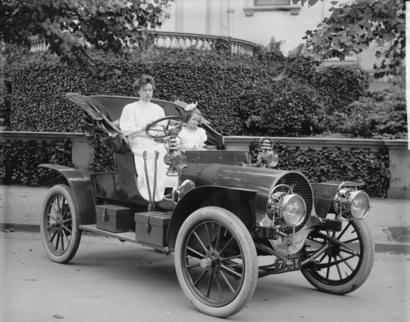
\includegraphics[width=\linewidth]{sample-franklin}
  \caption{1907 Franklin Model D roadster. Photograph by Harris \&
    Ewing, Inc. [Public domain], via Wikimedia
    Commons. (\url{https://goo.gl/VLCRBB}).}
  \Description{A woman and a girl in white dresses sit in an open car.}
\end{figure}

Your figures should contain a caption which describes the figure to
the reader.

Figure captions are placed {\itshape below} the figure.

Every figure should also have a figure description unless it is purely
decorative. These descriptions convey what’s in the image to someone
who cannot see it. They are also used by search engine crawlers for
indexing images, and when images cannot be loaded.

A figure description must be unformatted plain text less than 2000
characters long (including spaces).  {\bfseries Figure descriptions
  should not repeat the figure caption – their purpose is to capture
  important information that is not already provided in the caption or
  the main text of the paper.} For figures that convey important and
complex new information, a short text description may not be
adequate. More complex alternative descriptions can be placed in an
appendix and referenced in a short figure description. For example,
provide a data table capturing the information in a bar chart, or a
structured list representing a graph.  For additional information
regarding how best to write figure descriptions and why doing this is
so important, please see
\url{https://www.acm.org/publications/taps/describing-figures/}.

\subsection{The ``Teaser Figure''}

A ``teaser figure'' is an image, or set of images in one figure, that
are placed after all author and affiliation information, and before
the body of the article, spanning the page. If you wish to have such a
figure in your article, place the command immediately before the
\verb|\maketitle| command:
\begin{verbatim}
  \begin{teaserfigure}
    \includegraphics[width=\textwidth]{sampleteaser}
    \caption{figure caption}
    \Description{figure description}
  \end{teaserfigure}
\end{verbatim}

\section{Citations and Bibliographies}

The use of \BibTeX\ for the preparation and formatting of one's
references is strongly recommended. Authors' names should be complete
--- use full first names (``Donald E. Knuth'') not initials
(``D. E. Knuth'') --- and the salient identifying features of a
reference should be included: title, year, volume, number, pages,
article DOI, etc.

The bibliography is included in your source document with these two
commands, placed just before the \verb|\end{document}| command:
\begin{verbatim}
  \bibliographystyle{ACM-Reference-Format}
  \bibliography{bibfile}
\end{verbatim}
where ``\verb|bibfile|'' is the name, without the ``\verb|.bib|''
suffix, of the \BibTeX\ file.

Citations and references are numbered by default. A small number of
ACM publications have citations and references formatted in the
``author year'' style; for these exceptions, please include this
command in the {\bfseries preamble} (before the command
``\verb|\begin{document}|'') of your \LaTeX\ source:
\begin{verbatim}
  \citestyle{acmauthoryear}
\end{verbatim}

  Some examples.  A paginated journal article \cite{Abril07}, an
  enumerated journal article \cite{Cohen07}, a reference to an entire
  issue \cite{JCohen96}, a monograph (whole book) \cite{Kosiur01}, a
  monograph/whole book in a series (see 2a in spec. document)
  \cite{Harel79}, a divisible-book such as an anthology or compilation
  \cite{Editor00} followed by the same example, however we only output
  the series if the volume number is given \cite{Editor00a} (so
  Editor00a's series should NOT be present since it has no vol. no.),
  a chapter in a divisible book \cite{Spector90}, a chapter in a
  divisible book in a series \cite{Douglass98}, a multi-volume work as
  book \cite{Knuth97}, a couple of articles in a proceedings (of a
  conference, symposium, workshop for example) (paginated proceedings
  article) \cite{Andler79, Hagerup1993}, a proceedings article with
  all possible elements \cite{Smith10}, an example of an enumerated
  proceedings article \cite{VanGundy07}, an informally published work
  \cite{Harel78}, a couple of preprints \cite{Bornmann2019,
    AnzarootPBM14}, a doctoral dissertation \cite{Clarkson85}, a
  master's thesis: \cite{anisi03}, an online document / world wide web
  resource \cite{Thornburg01, Ablamowicz07, Poker06}, a video game
  (Case 1) \cite{Obama08} and (Case 2) \cite{Novak03} and \cite{Lee05}
  and (Case 3) a patent \cite{JoeScientist001}, work accepted for
  publication \cite{rous08}, 'YYYYb'-test for prolific author
  \cite{SaeediMEJ10} and \cite{SaeediJETC10}. Other cites might
  contain 'duplicate' DOI and URLs (some SIAM articles)
  \cite{Kirschmer:2010:AEI:1958016.1958018}. Boris / Barbara Beeton:
  multi-volume works as books \cite{MR781536} and \cite{MR781537}. A
  couple of citations with DOIs:
  \cite{2004:ITE:1009386.1010128,Kirschmer:2010:AEI:1958016.1958018}. Online
  citations: \cite{TUGInstmem, Thornburg01, CTANacmart}. Artifacts:
  \cite{R} and \cite{UMassCitations}.

\section{Acknowledgments}

Identification of funding sources and other support, and thanks to
individuals and groups that assisted in the research and the
preparation of the work should be included in an acknowledgment
section, which is placed just before the reference section in your
document.

This section has a special environment:
\begin{verbatim}
  \begin{acks}
  ...
  \end{acks}
\end{verbatim}
so that the information contained therein can be more easily collected
during the article metadata extraction phase, and to ensure
consistency in the spelling of the section heading.

Authors should not prepare this section as a numbered or unnumbered {\verb|\section|}; please use the ``{\verb|acks|}'' environment.

\section{Appendices}

If your work needs an appendix, add it before the
``\verb|\end{document}|'' command at the conclusion of your source
document.

Start the appendix with the ``\verb|appendix|'' command:
\begin{verbatim}
  \appendix
\end{verbatim}
and note that in the appendix, sections are lettered, not
numbered. This document has two appendices, demonstrating the section
and subsection identification method.

\section{SIGCHI Extended Abstracts}

The ``\verb|sigchi-a|'' template style (available only in \LaTeX\ and
not in Word) produces a landscape-orientation formatted article, with
a wide left margin. Three environments are available for use with the
``\verb|sigchi-a|'' template style, and produce formatted output in
the margin:
\begin{itemize}
\item {\verb|sidebar|}:  Place formatted text in the margin.
\item {\verb|marginfigure|}: Place a figure in the margin.
\item {\verb|margintable|}: Place a table in the margin.
\end{itemize}

%%
%% The acknowledgments section is defined using the "acks" environment
%% (and NOT an unnumbered section). This ensures the proper
%% identification of the section in the article metadata, and the
%% consistent spelling of the heading.
\begin{acks}
To Robert, for the bagels and explaining CMYK and color spaces.
\end{acks}

%%
%% The next two lines define the bibliography style to be used, and
%% the bibliography file.
\bibliographystyle{ACM-Reference-Format}
\bibliography{sample-base}

%%
%% If your work has an appendix, this is the place to put it.
\appendix

\section{Research Methods}

\subsection{Part One}

Lorem ipsum dolor sit amet, consectetur adipiscing elit. Morbi
malesuada, quam in pulvinar varius, metus nunc fermentum urna, id
sollicitudin purus odio sit amet enim. Aliquam ullamcorper eu ipsum
vel mollis. Curabitur quis dictum nisl. Phasellus vel semper risus, et
lacinia dolor. Integer ultricies commodo sem nec semper.

\subsection{Part Two}

Etiam commodo feugiat nisl pulvinar pellentesque. Etiam auctor sodales
ligula, non varius nibh pulvinar semper. Suspendisse nec lectus non
ipsum convallis congue hendrerit vitae sapien. Donec at laoreet
eros. Vivamus non purus placerat, scelerisque diam eu, cursus
ante. Etiam aliquam tortor auctor efficitur mattis.

\section{Online Resources}

Nam id fermentum dui. Suspendisse sagittis tortor a nulla mollis, in
pulvinar ex pretium. Sed interdum orci quis metus euismod, et sagittis
enim maximus. Vestibulum gravida massa ut felis suscipit
congue. Quisque mattis elit a risus ultrices commodo venenatis eget
dui. Etiam sagittis eleifend elementum.

Nam interdum magna at lectus dignissim, ac dignissim lorem
rhoncus. Maecenas eu arcu ac neque placerat aliquam. Nunc pulvinar
massa et mattis lacinia.

\end{document}
\endinput
%%
%% End of file `sample-manuscript.tex'.
